\documentclass{report}
\usepackage{longtable}
\usepackage{booktabs}
\usepackage{graphicx}
\usepackage[pdfauthor={Kristoffer Nordstroem},%
pdftitle={Architecture specification for pymergevcd},%
pdfsubject={Architecture specification for pymergevcd},%
pdfkeywords={merge vcd files},%
pagebackref=true,%
pdftex, bookmarks=true, colorlinks=true]{hyperref}

\usepackage[a4paper]{geometry}
\usepackage[titles]{tocloft}
\usepackage{fancyhdr}

\setlength{\cftsubsecnumwidth}{4em}
\pagestyle{fancy}
\fancyhead{}
\fancyfoot{}
\fancyhead[L]{\rightmark}
\fancyfoot[R]{\thepage}
\fancyfoot[L]{Version \input{../artifacts/reqs-version.txt}}
\renewcommand{\headrulewidth}{0.4pt}
\renewcommand{\footrulewidth}{0.4pt}

\parindent0em

\begin{document}
\thispagestyle{empty}

\title{Software Architecture and Design Specification}
\author{Kristoffer Nordström}
\date{\today}
\maketitle
\newpage

\tableofcontents

\listoffigures
\listoftables

\newpage

\chapter{Software Architecture Specification}

The architecture in Fig.\ \ref{fig:architecture} defines the building blocks and encapsulates the volatility of the system.

\begin{figure}
  \centering
  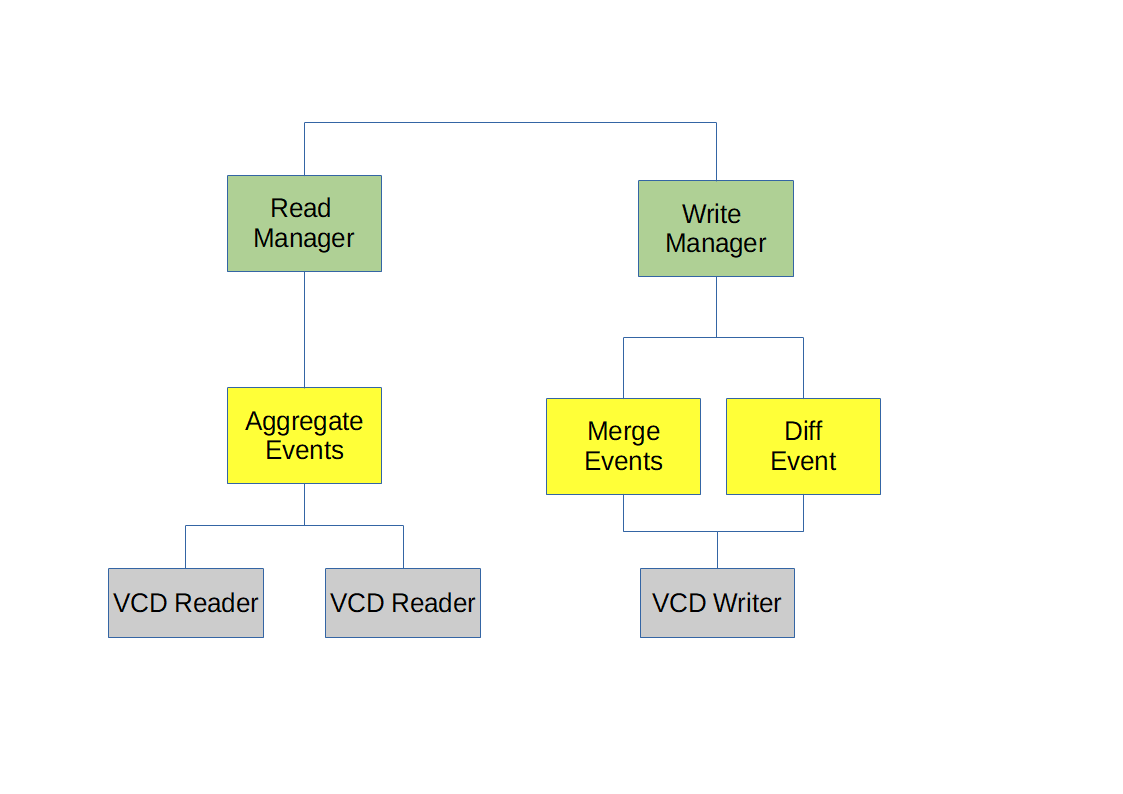
\includegraphics[width=1.0\textwidth]{latex/architecture.png}
  \caption{The Architecture}
  \label{fig:architecture}
\end{figure}


% Output topic 'ReqsDocument'


\chapter{Software Requirements Specification}

This document describes the requirements defined for \emph{pymergevcd}.

\paragraph{VCD Merger}

\hypertarget{SW-RS-1}{SW-RS-1} 
\label{SW-RS-1}

Merge multiple files

\textbf{Rationale:} compare files visually

\textbf{Note:} 

 \textbf{Solved by:}
 \hyperlink{SW-RS-100}{SW-RS-100}  \hyperlink{SW-RS-110}{SW-RS-110} 






\par{\small \begin{center}
\begin{tabular}{rlrlrl}
   Id: & SW-RS-1               & Priority: & 0.0          & Owner: & customers \\
   Invented on: & 2019-12-15 & Invented by: & default & Status: & not done \\
   Class: & detailable & Hash: & 7d6734f3
\end{tabular}\end{center}
}

\paragraph{Merge Two Files}

\hypertarget{SW-RS-100}{SW-RS-100} 
\label{SW-RS-100}

Merge two VCD files into one with a separate namespace for each file.

\textbf{Rationale:} 

\textbf{Note:} 

 \textbf{Solved by:}
 \hyperlink{SW-RS-101}{SW-RS-101} 


 \textbf{Depends on:}
 \hyperlink{SW-RS-1}{SW-RS-1} 




\par{\small \begin{center}
\begin{tabular}{rlrlrl}
   Id: & SW-RS-100               & Priority: & 0.0          & Owner: & customers \\
   Invented on: & 2019-12-15 & Invented by: & default & Status: & not done \\
   Class: & detailable & Hash: & d4b3ef7c
\end{tabular}\end{center}
}

\paragraph{Merge Multiple Files}

\hypertarget{SW-RS-101}{SW-RS-101} 
\label{SW-RS-101}

Merge multiple VCD files into one with a separate namespace for each file.

\textbf{Rationale:} 

\textbf{Note:} 



 \textbf{Depends on:}
 \hyperlink{SW-RS-100}{SW-RS-100} 




\par{\small \begin{center}
\begin{tabular}{rlrlrl}
   Id: & SW-RS-101               & Priority: & 0.0          & Owner: & customers \\
   Invented on: & 2019-12-15 & Invented by: & default & Status: & not done \\
   Class: & detailable & Hash: & aef93153
\end{tabular}\end{center}
}

\paragraph{Merge-Diff Two Files}

\hypertarget{SW-RS-110}{SW-RS-110} 
\label{SW-RS-110}

Merge two VCD files with the second as a xor-diff relative to the first

\textbf{Rationale:} Find differences quickly

\textbf{Note:} 



 \textbf{Depends on:}
 \hyperlink{SW-RS-1}{SW-RS-1} 




\par{\small \begin{center}
\begin{tabular}{rlrlrl}
   Id: & SW-RS-110               & Priority: & 0.0          & Owner: & customers \\
   Invented on: & 2019-12-15 & Invented by: & default & Status: & not done \\
   Class: & detailable & Hash: & 81d53eed
\end{tabular}\end{center}
}


\appendix
%% Traceability Matrix



\chapter{Traceability Matrix}


\begin{longtable}{l c  c }
\caption{Traceability Matrix Table} \\
\label{tbl:tracematrix} \\
\toprule
Req. ID  & Status 
 & UT  \\
\midrule
\endfirsthead
\toprule
Req. ID  & Status 
 & UT  \\
\midrule
\endhead
\bottomrule
\endfoot
\bottomrule
\endlastfoot

% Output topic 'ReqsDocument'
% Software Design Specification 

\hyperref[SW-AS-1]{SW-AS-1} \label{trmat:SW-AS-1} & %
passed %
 & passed  %
 \\
%%% TRACEMAT_RID_FINE : SW-AS-1

\hyperref[SW-AS-100]{SW-AS-100} \label{trmat:SW-AS-100} & %
open %
 & open  %
 \\
%%% TRACEMAT_RID_FINE : SW-AS-100

\hyperref[SW-AS-101]{SW-AS-101} \label{trmat:SW-AS-101} & %
open %
 & open  %
 \\
%%% TRACEMAT_RID_FINE : SW-AS-101

\hyperref[SW-AS-102]{SW-AS-102} \label{trmat:SW-AS-102} & %
open %
 & open  %
 \\
%%% TRACEMAT_RID_FINE : SW-AS-102

\hyperref[SW-AS-200]{SW-AS-200} \label{trmat:SW-AS-200} & %
passed %
 & passed  %
 \\
%%% TRACEMAT_RID_FINE : SW-AS-200

\hyperref[SW-AS-201]{SW-AS-201} \label{trmat:SW-AS-201} & %
passed %
 & passed  %
 \\
%%% TRACEMAT_RID_FINE : SW-AS-201

\hyperref[SW-AS-202]{SW-AS-202} \label{trmat:SW-AS-202} & %
passed %
 & passed  %
 \\
%%% TRACEMAT_RID_FINE : SW-AS-202

\hyperref[SW-AS-300]{SW-AS-300} \label{trmat:SW-AS-300} & %
passed %
 & passed  %
 \\
%%% TRACEMAT_RID_FINE : SW-AS-300

\hyperref[SW-AS-301]{SW-AS-301} \label{trmat:SW-AS-301} & %
open %
 & open  %
 \\
%%% TRACEMAT_RID_FINE : SW-AS-301

\hyperref[SW-AS-302]{SW-AS-302} \label{trmat:SW-AS-302} & %
open %
 & open  %
 \\
%%% TRACEMAT_RID_FINE : SW-AS-302

\hyperref[SW-AS-500]{SW-AS-500} \label{trmat:SW-AS-500} & %
passed %
 & passed  %
 \\
%%% TRACEMAT_RID_FINE : SW-AS-500

\hyperref[SW-AS-501]{SW-AS-501} \label{trmat:SW-AS-501} & %
passed %
 & passed  %
 \\
%%% TRACEMAT_RID_FINE : SW-AS-501

\end{longtable}


\end{document}
